\subsection{Independent Evaluation: Timely Attribution and Alarm Cost}
\label{sec:c01-results}

The five-model bank makes \COneMixTimely{}/\COneMixTotal{} timely
family-and-source decisions with \COneMixExtras{} unmatched alarms on
event records, and its nominal counterpart \COneNomTimely{}/\COneNomTotal{}
with \COneNomExtras{}. These are paired replays of 108 interventions in 18
physical parents, not 648 independent events. On the 72 normal records
(42{,}336\,s, 11.8\,h of monitored time per method) neither bank raises an
alarm, which bounds the normal false-alarm rate below 0.26 per hour at 95\%
confidence (Poisson). Every matched diagnosis emitted before OFF names the
correct family and source; the timely misses are late or absent
diagnoses. Table~\ref{tab:c01-direct} and Fig.~\ref{fig:c01-main} give the
family split.

\begin{table}[t]\centering\small
\caption{Held-out continuous-stream decisions. Each family has 324 replays
of 54 distinct interventions; extras are unmatched alarms on event records.
The ExtraTrees adapters keep their original operating points.}
\label{tab:c01-direct}
\begin{tabular}{@{}lrrr@{}}\toprule
Method & Load & Line & Extras\\\midrule
Physical bank & \ReaderPhysicalLoad/324 & \ReaderPhysicalLine/324 & \COneMixExtras\\
Nominal bank & \ReaderNominalLoad/324 & \ReaderNominalLine/324 & \COneNomExtras\\
ExtraTrees & \ReaderETLoad/324 & \ReaderETLine/324 & \COneETExtras\\
ExtraTrees short & \ReaderETShortLoad/324 & \ReaderETShortLine/324 & \ReaderETShortExtras\\\bottomrule
\end{tabular}\end{table}

\begin{figure*}[t]\centering
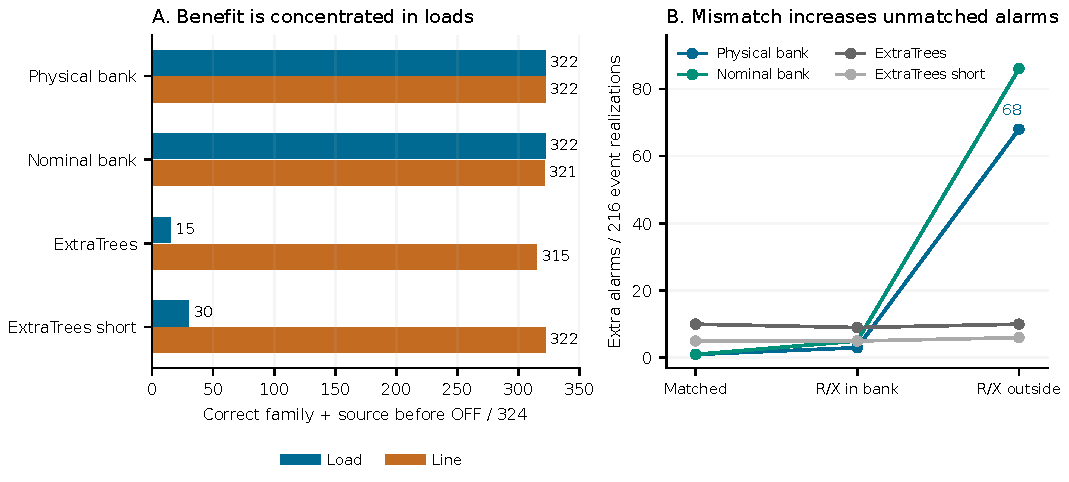
\includegraphics[width=.91\textwidth]{figures/generated/reader_c01_tradeoff.pdf}
\caption{Held-out continuous evaluation. (A) Timely correct family and source
by event family, with 324 paired replays per family. (B) Unmatched alarms on
event records for the two noise levels of each R/X condition (216 event
replays per condition). Each method keeps its own publication rule.}
\label{fig:c01-main}\end{figure*}

The extra alarms concentrate where the network model is wrong: 68 of the
72 occur when the true R/X perturbation lies outside the five-model bank,
68 alarms in 1.08\,h of out-of-bank monitored event-record time (about 63
per hour), against four in the other four strata together. Out-of-bank mismatch also produces the only
four timely misses. The supplement gives the paired parent-cluster
intervals; the physical bank's median alarm delay is about 0.27\,s in the
matched and in-bank conditions, comparable to the learned adapters
(0.19--0.30\,s).

We compare these delays retrospectively with Prediction~1. For the nominal bank on matched networks,
line alarms arrive after a median \RevObsLineDelay\,s, at the six-report
confirmation floor of \RevPredAlarmDelay\,s less the sub-report onset
phase, and doubling the noise leaves them unchanged. Load alarms arrive
after \RevObsLoadDelay\,s, again unchanged by doubled noise but about
\RevLoadExcessReports{} reports after the nominal signature reference crossing. Line delays are
consistent with the publication floor, while load delays exceed that
model-based reference.
The two ExtraTrees adapters recover lines (\ReaderETLine{} and
\ReaderETShortLine{} of 324) but few loads (\ReaderETLoad{} and
\ReaderETShortLoad{}). The diagnosis-time distributions in the supplement show that this is a
coverage failure: every load diagnosis the adapters do emit before OFF is
correct, but most load interventions receive none. A per-report audit on
four further matched records (12 load and 12 line interventions,
1{,}245 and 1{,}143 in-event reports) locates the failure before any
publication rule. During every load intervention the reference model's
per-report argmax is the normal class in all reports, and the median of
the largest true-class score is 0.09; during line interventions the true
line wins 96\% of the reports with median peak score 0.93. The short-window
variant ranks the true load first in only 2 of 12 load interventions. The
learned representation thus does not separate 3--14\% load changes from
normal operation, whereas the nominal physical signatures have large separation energies
for the same changes (Fig.~\ref{fig:theory-information}). The same pattern was already present in
their development validation (Section~\ref{sec:narrative-protocol}), so the
comparison shows that the physical bank recovers load interventions that
these particular adapters miss; it is not a test of the best attainable
learned detector at a common alarm budget.
In the persistent-line test, both banks and both adapters identify the
correct line first on all 162 openings. The adapter of Chen \emph{et al.}'s
quickest-change detector identifies 74/162; 66 records stop before the
opening and 22 afterward on a wrong line, and it stops on all 72 paired
normal records (first stop after 2{,}522\,s of cumulative normal exposure,
against 42{,}336\,s monitored without alarm by the other methods). Its
white-injection, quasi-static model does not describe the colored,
dynamically filtered measurements of this plant, so its threshold is far
from its nominal false-alarm rate. We therefore read this result as a test
of transfer under model mismatch, not as a ranking of quickest-change
detection. After the first identification, the two learned adapters raise
\PersistETExtras{} and \PersistShortExtras{} further unmatched alarms on the
same persistent records, against \PersistPhysicalExtras{} for the
physical bank. Stratified tables, failure ledgers, restoration outcomes and
censoring are in the supplement.

Table~\ref{tab:competition-metrics} restates the evaluation in the metrics
prescribed by the competition guide. Per-report detection F1 is 0.91 for
the bank and 0.58--0.64 for the learned adapters, whose precision is higher
because they alarm only on the line interventions. None of the methods
raises an alarm on the normal records. The bank has no trained weights:
its parameters are the network model, the noise model estimated from normal
data, and a few prior and publication constants fixed during
development. The nominal bank processes one
minute of PMU data in 48\,s on one CPU thread.
\begin{table*}[t]\centering\small
\caption{Independent evaluation in the metric vocabulary of the competition guide (648 interventions, 706\,min of normal records, three R/X conditions pooled). Detection is scored per report; Top-$k$ requires the correct family and source among the first $k$ candidates. Run time is per minute of PMU data on one CPU thread.}
\label{tab:competition-metrics}
\begin{tabular}{@{}lrrrrrrrr@{}}\toprule
Method & Precision & Recall & F1 & FA/min & Delay (s) & Top-1 & Top-3 & Run time (s/min)\\\midrule
Physical bank, five R/X models & 0.888 & 0.926 & 0.907 & 0 & 0.20 & 0.995 & 0.995 & 179\\
Physical bank, nominal model & 0.874 & 0.927 & 0.900 & 0 & 0.27 & 0.995 & 0.995 & 48\\
Submitted ExtraTrees & 0.938 & 0.424 & 0.584 & 0 & 0.27 & 0.509 & 0.509 & --\\
Retrained short-window ExtraTrees & 0.944 & 0.483 & 0.639 & 0 & 0.19 & 0.543 & 0.543 & --\\
\bottomrule\end{tabular}\end{table*}

